% espaces verticaux des formules centrées : valeurs fixes (sans étirement ni compression), pour que les blocs ne bougent pas d'un overlay à l'autre
\newcommand{\rigiddisplayskips}[1]{\setlength{\abovedisplayskip}{#1}\setlength{\belowdisplayskip}{#1}\setlength{\abovedisplayshortskip}{#1}\setlength{\belowdisplayshortskip}{#1}}

\SectionNote{$\bm{\mu}$ is fixed and omitted from the notation: basis, dofs and solution are valid for this $\bm{\mu}$ only}
\section[PINN]{Non-parametric enrichment (PINN loss)}

\begin{frame}{Neural-enriched Galerkin scheme}
	\rigiddisplayskips{7pt}
	\centering
	\only<1>{
\includegraphics[page=1]{images/contrib2/learnable_scheme/learnable_scheme.pdf}}%
	\only<2>{
\includegraphics[page=2]{images/contrib2/learnable_scheme/learnable_scheme.pdf}}%
	\only<3>{
\includegraphics[page=3]{images/contrib2/learnable_scheme/learnable_scheme.pdf}}%
	\only<4->{
\includegraphics[page=4]{images/contrib2/learnable_scheme/learnable_scheme.pdf}}

	\vspace{10pt}
	\raggedright
	\textbf{Neural network:} Construct a single neural network $v_\theta(\bm{x})$ on $\Omega$ (with $N_\theta$ weights), shared by all cells.

	\vspace{4pt}
	\blk{2}{%
		\textbf{Enriched basis:} Construct a multiplier $m_\theta(\bm{x})$ from $v_\theta(\bm{x})$ and define the \coloredonly<2>{enriched basis functions}\footnote{can be adapted to CG using the connectivity table} as:
		\vspace{-3pt}
		\[
			\phi^\theta_{c,i}(\bm{x})=m_\theta(\bm{x})\,\phi_{c,i}(\bm{x}).
		\]
	}

	\vspace{-3pt}
	\blk{3}{%
	\textbf{Galerkin scheme ($\bm{\mu}$ fixed):} Solve the linear system:
	\vspace{-3pt}
	\[
		\bm{R}_h\big(\bm{\beta}_h(\coloredonly<3>{\theta});\coloredonly<3>{\theta}\big)=A_h(\coloredonly<3>{\theta})\,\bm{\beta}_h(\coloredonly<3>{\theta})-\bm{b}_h(\coloredonly<3>{\theta})=\bm{0},
	\]
	with \hspace{30pt} $
		A_{(c,i),(c',j)}(\theta)=a_h^{\text{disc}}(\phi^\theta_{c',j},\phi^\theta_{c,i}), \qquad b_{(c,i)}(\theta)=l(\phi^\theta_{c,i}).$
	}

	\vspace{4pt}
	\blk*{4}{%
		\textbf{Solution:} Reconstruct the solution in the enriched space as:
		\vspace{-3pt}
		\[
			u_{h,\theta}(\bm{x})=\sum_{c,i}\beta_{c,i}(\theta)\,\coloredonly<4>{\phi^\theta_{c,i}}(\bm{x}).
		\]
	}
\end{frame}

\begin{frame}{Learning $\theta$: differentiating through the solver}
	\rigiddisplayskips{7pt}
	\centering
	\only<1>{
\includegraphics[page=5]{images/contrib2/learnable_scheme/learnable_scheme.pdf}}%
	\only<2->{
\includegraphics[page=6]{images/contrib2/learnable_scheme/learnable_scheme.pdf}}

	\vspace{-8pt}
	\raggedright
	\textbf{Bi-level problem:} Learn $\theta$ so that the Galerkin solution $u_{h,\theta}$ minimizes $\mathcal{J}$:
	\vspace{-3pt}
	\[
		\theta^\star=\argmin\nolimits_\theta\,\mathcal{J}(\bm{\beta}_h(\theta);\theta) \quad \text{s.t.} \quad \bm{R}_h(\bm{\beta}_h(\theta);\theta)=\bm{0}
	\]

	\vspace{-3pt}
	\blk{2}{%
	\textbf{Gradient:} Differentiate \coloredonly<2>{through the solver} (chain rule):
	\vspace{-3pt}
	\[
		\frac{d\mathcal{J}}{d\theta}=\underbrace{\frac{\partial\mathcal{J}}{\partial\theta}\bigg|_{\bm{\beta}_h}}_{\text{direct}}+\underbrace{\coloredonly<3>{\frac{\partial\mathcal{J}}{\partial\bm{\beta}_h}\cdot\frac{d\bm{\beta}_h}{d\theta}}}_{\text{through the dofs}}
	\]
	}

	\vspace{-3pt}
	\blk*{3}{%
	\textbf{Adjoint:} With a gradient-based optimizer, avoid $d\bm{\beta}_h/d\theta$ (only \coloredonly<3>{one} linear solve, whatever $N_\theta$):
	\vspace{-3pt}
	\[
		A_h(\theta)^T\bm{\lambda}_h=\left(\frac{\partial\mathcal{J}}{\partial\bm{\beta}_h}\right)^T \;\Rightarrow\; \frac{d\mathcal{J}}{d\theta}=\frac{\partial\mathcal{J}}{\partial\theta}\bigg|_{\bm{\beta}_h}-\bm{\lambda}_h^T\,\frac{\partial\bm{R}_h}{\partial\theta}(\bm{\beta}_h;\theta)
	\]
	}
\end{frame}

\begin{frame}{1D test case and PINN loss}
	\rigiddisplayskips{7pt}
	\raggedright
	\textbf{Test case:} 1D advection-diffusion with a \coloredonly<1>{boundary layer}, $\Omega=(0,1)$, $\text{Pe}=20$, $f=1$:
	\vspace{-3pt}
	\[
		\left\{
		\begin{aligned}
			-\frac{1}{\text{Pe}}\,\partial_{xx}u+\bm{C}\,\partial_xu & =f &  & \text{in } \Omega, \\
			u                                                        & =0 &  & \text{on } \Gamma,
		\end{aligned}
		\right.
		\qquad \bm{C}(x,\bm{\mu})=\mu_1+\mu_2x
	\]
	with $\bm{\mu}=(\mu_1,\mu_2)=(0.8,0.8)$ fixed.

	\vspace{2pt}
	\blk{2}{%
		\textbf{PINN loss:} Minimize \coloredonly<2>{residual and boundary terms} ($\omega_r=1$, $\omega_b=10$):
		\vspace{-3pt}
		\[
			\mathcal{J}(\theta)=\omega_r\underbrace{\int_\Omega\Big|-\frac{1}{\text{Pe}}\,\partial_{xx}\coloredonly<3>{u_{h,\theta}}+(\mu_1+\mu_2x)\,\partial_x\coloredonly<3>{u_{h,\theta}}-f\Big|^2\mathrm{d}\bm{x}}_{\mathcal{J}_r\ \text{(Monte Carlo, redrawn each epoch)}}+\;\omega_b\underbrace{\int_\Gamma\big|\coloredonly<3>{u_{h,\theta}}\big|^2\mathrm{d}\bm{x}}_{\mathcal{J}_b}
		\]
	}

	\vspace{-3pt}
	\blk{3}{%
		\textbf{Validity:} Learned for \coloredonly<3>{this configuration only}:
		\[
			\text{new} \; \bm{\mu}, \; k \; \text{or} \; N_\text{cells} \; \Rightarrow \; \text{new training}.
		\]
	}

	\vspace{4pt}
	\blk*{4}{%
		\textbf{Evaluation:} Relative $L^2$ error w.r.t.\ a reference FEM solution ($128$ cells, $\mathbb{Q}_4$), \coloredonly<4>{never used in the training}.
	}
\end{frame}

\begin{frame}{Learned basis: affine multiplier}
	\raggedright
	\textbf{Setting:} CG, $N_\text{cells}=4$ cells, $\mathbb{Q}_3$ ($N_\text{dofs}=13$), affine multiplier $m_\theta=2+0.1\,v_\theta$. %best of $20$ seeds.

	\textbf{Training:} MLP $v_\theta$ (tanh, $2\times16$, $N_\theta=321$), ENG optimizer\myfootcite{Muller2023}, $300$ epochs, $6000$ collocation points.

	\vspace{2pt}
	\centering
	\only<1>{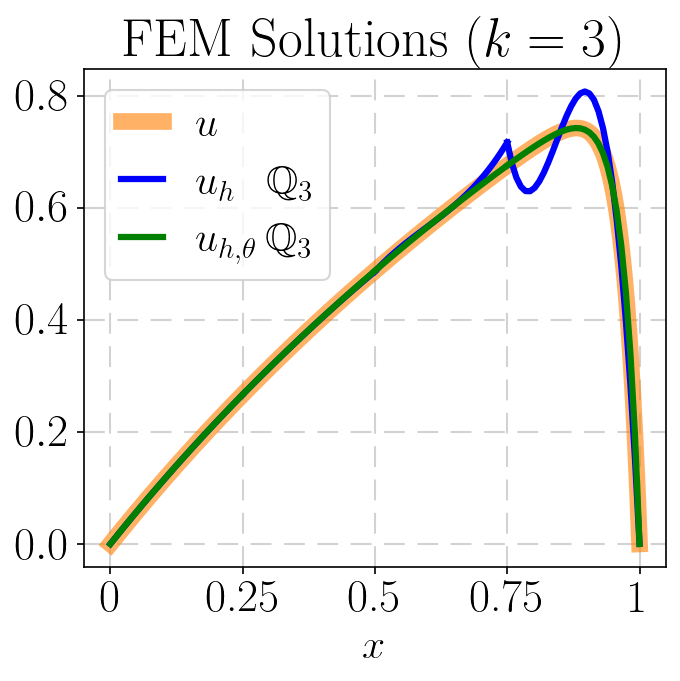
\includegraphics[height=4.2cm]{images/contrib2/first_study/solution_Q3.png}\hspace{1cm}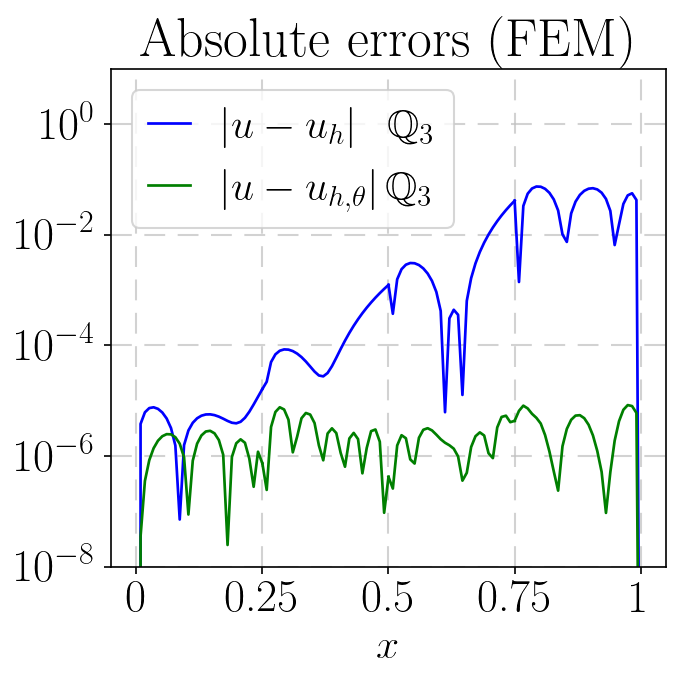
\includegraphics[height=4.2cm]{images/contrib2/first_study/error_Q3.png}}%
	\only<2->{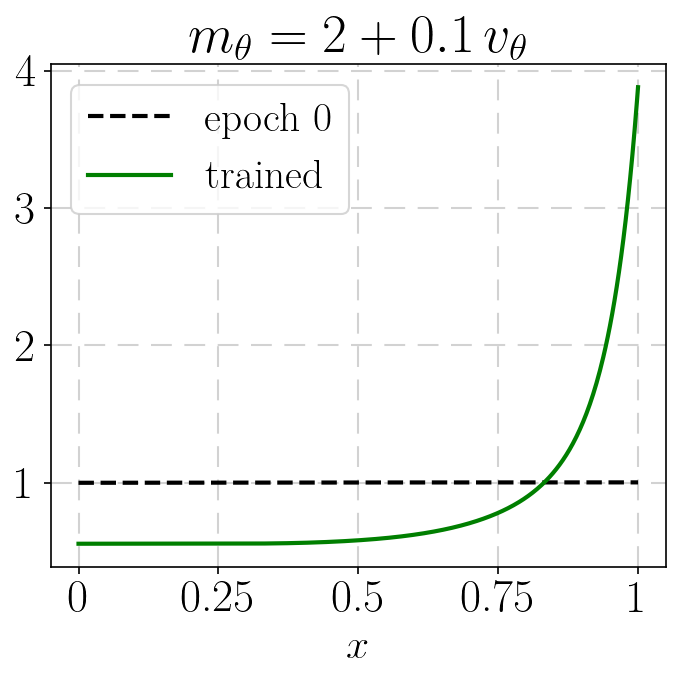
\includegraphics[height=4.2cm]{images/contrib2/first_study/multiplier_Q3.png}\hspace{0.5cm}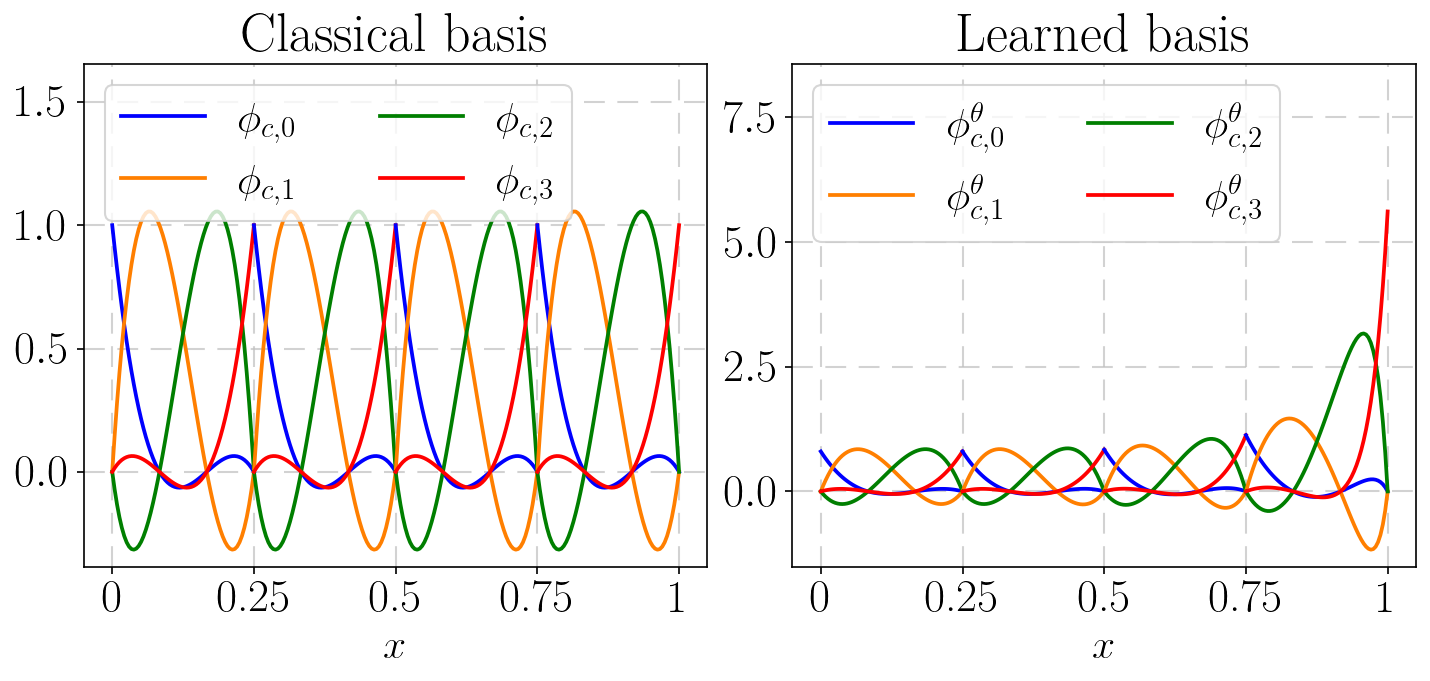
\includegraphics[height=4.2cm]{images/contrib2/first_study/bases_Q3.png}}

	\vspace{2pt}
	\raggedright
	\textbf{Solutions:} Classical $u_h$ \coloredonly<1>{oscillates} in the boundary layer, $u_{h,\theta}$ matches the reference ($\sim\!10^{-5}$ against $7\cdot10^{-2}$).

	\blk*{2}{%
		\textbf{Basis:} The multiplier grows in the \coloredonly<2>{boundary layer}: the last basis functions are amplified.
	}

\end{frame}

\begin{frame}{Choice of the multiplier}
	\vspace{-5pt}
	\coloredonly<1>{Fix $N_\text{dofs}=25$ and $N_\theta\in\{134,\dots,151\}$, vary the levers}: $(N_\text{cells},k)$ and the MLP shape (width, depth).

	\vspace{2pt}
	$20$ configurations $\times$ $20$ seeds $=400$ trainings per multiplier ($100$ epochs, $5000$ collocation points).

	\begin{minipage}[t]{0.39\linewidth}
		\vspace{4pt}
		\blk{2}{%
			\textbf{Affine multiplier:}
			\vspace{-4pt}
			$$m_\theta=2+0.1\,v_\theta$$
		}

		\vspace{-4pt}
		\blk{3}{%
			\textbf{Diagnosis:}

			Some trainings \coloredonly<3>{explode} (loss $=$ NaN).

			\vspace{2pt}
			Steps and sign changes never beat FEM.
		}

		\vspace{6pt}
		\blk*{4}{%
			\textbf{Fix:} \coloredonly<4>{Positive multiplier}
			\vspace{-4pt}
			$$m_\theta=\text{exp}(2\,\text{tanh}\, v_\theta)$$

			\vspace{-4pt}
			with \coloredonly<4>{bounded weights}:

			No sign change, no step.
		}
	\end{minipage}
	\hfill
	\begin{minipage}[t]{0.59\linewidth}
		\vspace{-8pt}
		\centering
		\only<2>{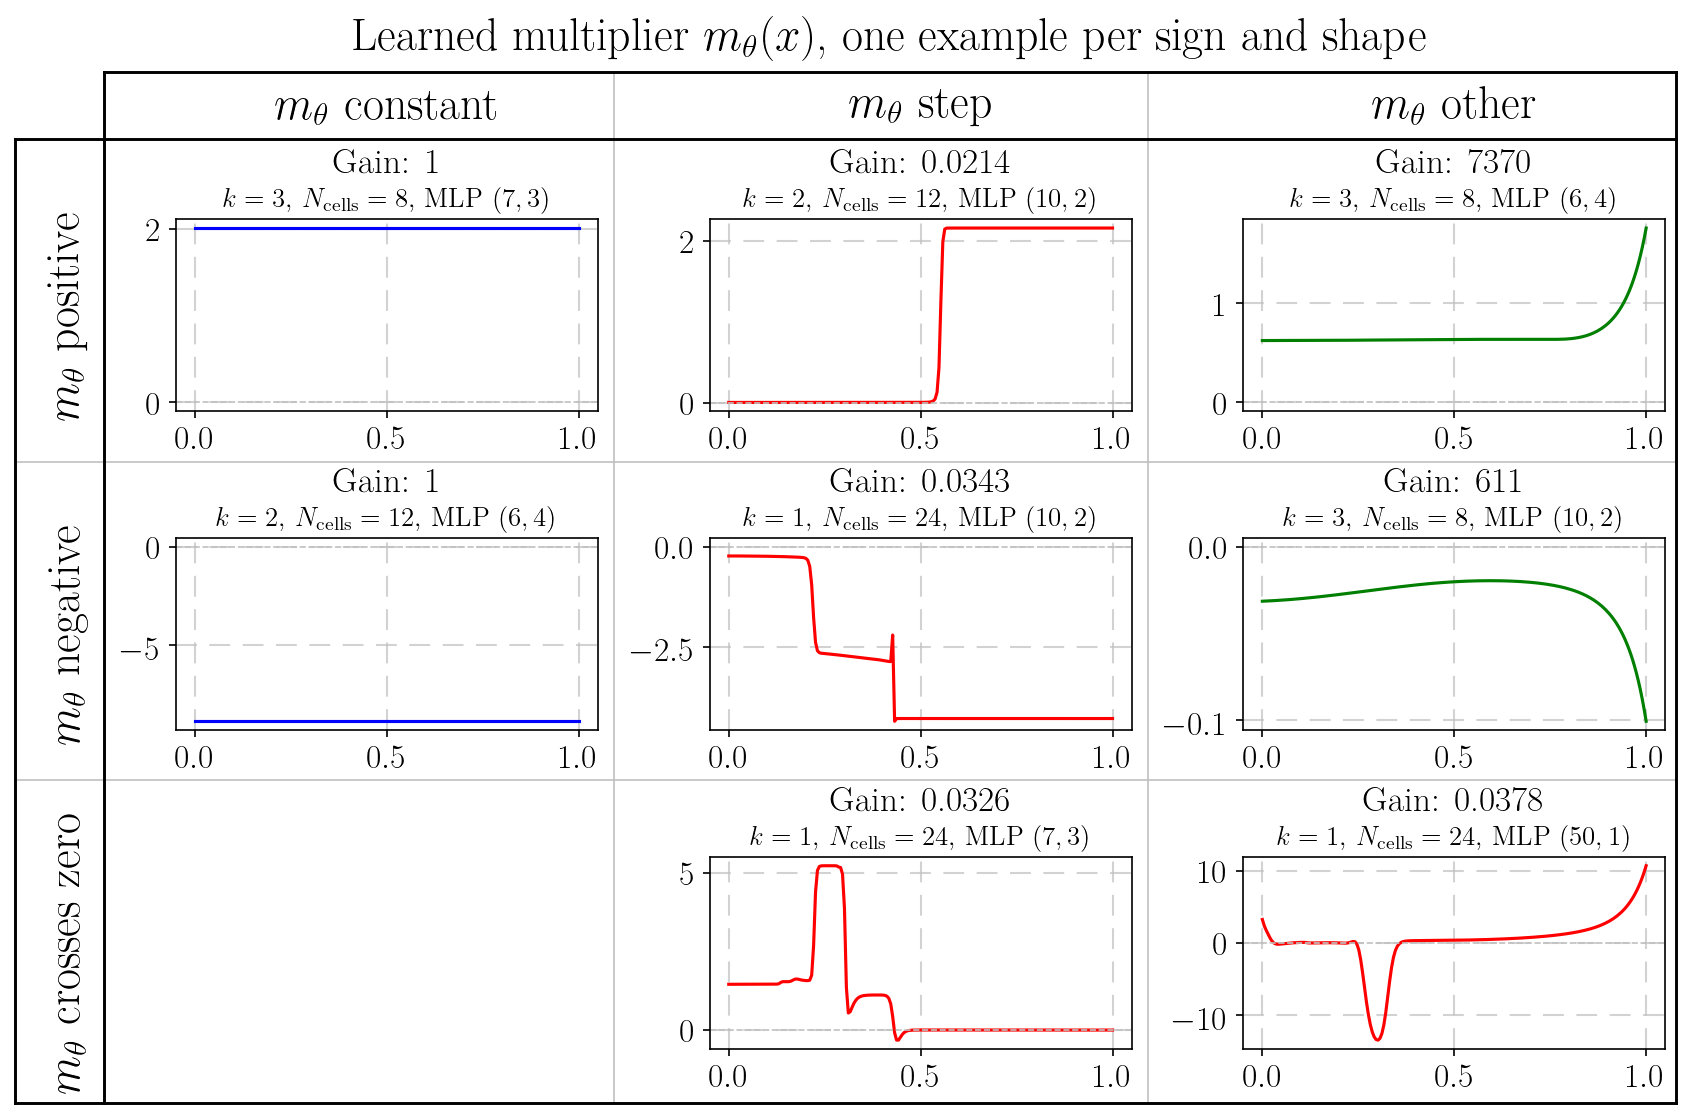
\includegraphics[width=\linewidth]{images/contrib2/multiplier/m_profiles_affine.png}}%
		\only<3>{\vspace{12pt}
			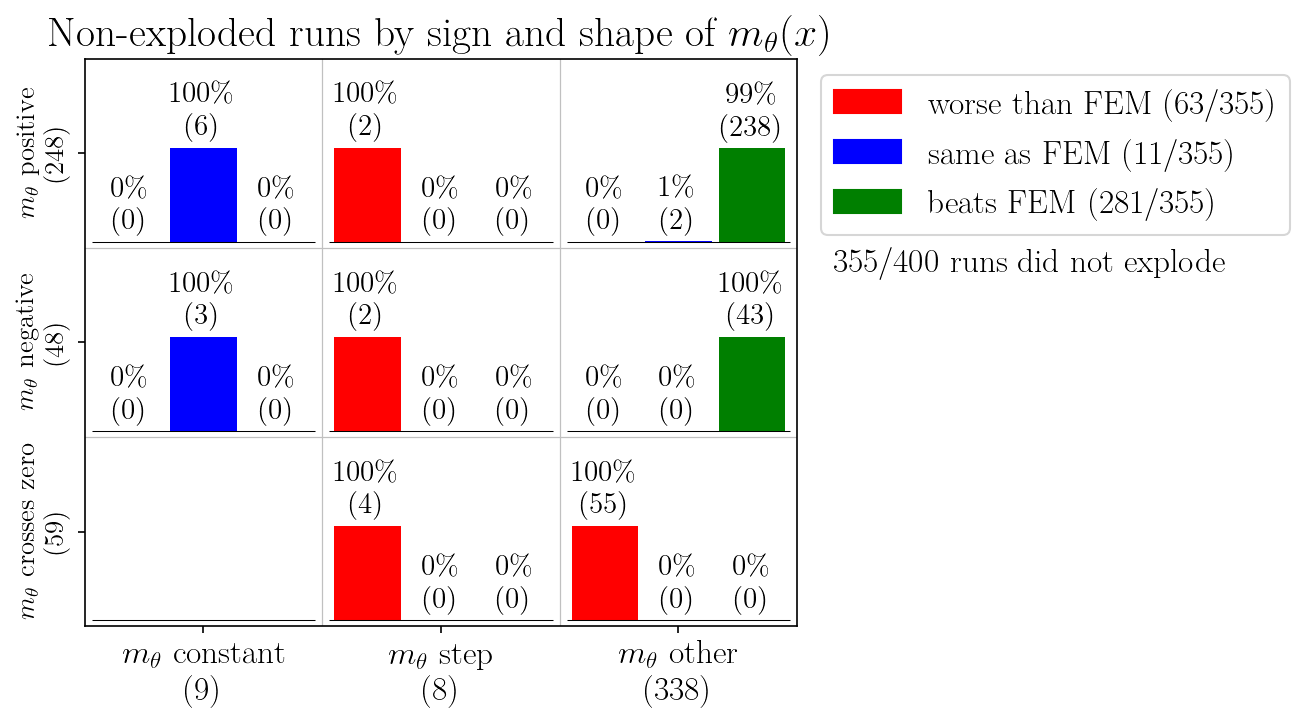
\includegraphics[width=\linewidth]{images/contrib2/multiplier/shape_sign_affine.png}}%
		\only<4->{\vspace{12pt}
			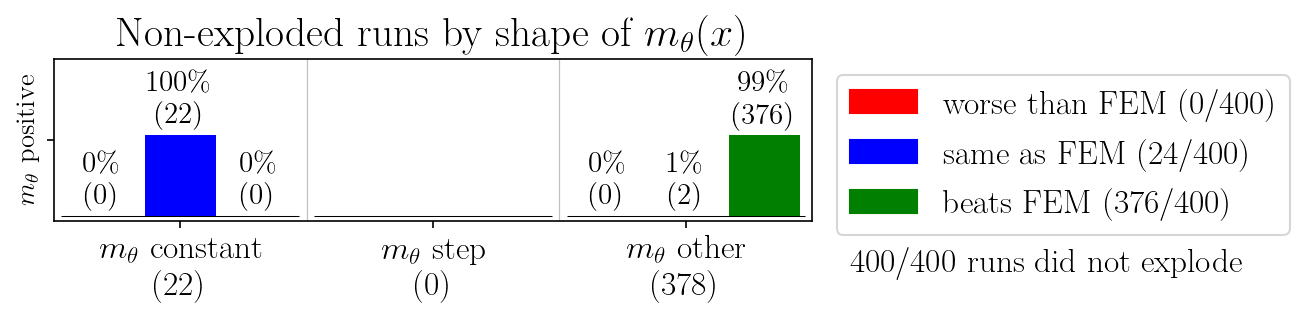
\includegraphics[width=\linewidth]{images/contrib2/multiplier/shape_sign_bounded.png}}%
	\end{minipage}
\end{frame}

\begin{frame}{Results at fixed budget}
	\vspace{-8pt}
	\parbox[t][5.2cm][c]{\linewidth}{\centering
		\only<1>{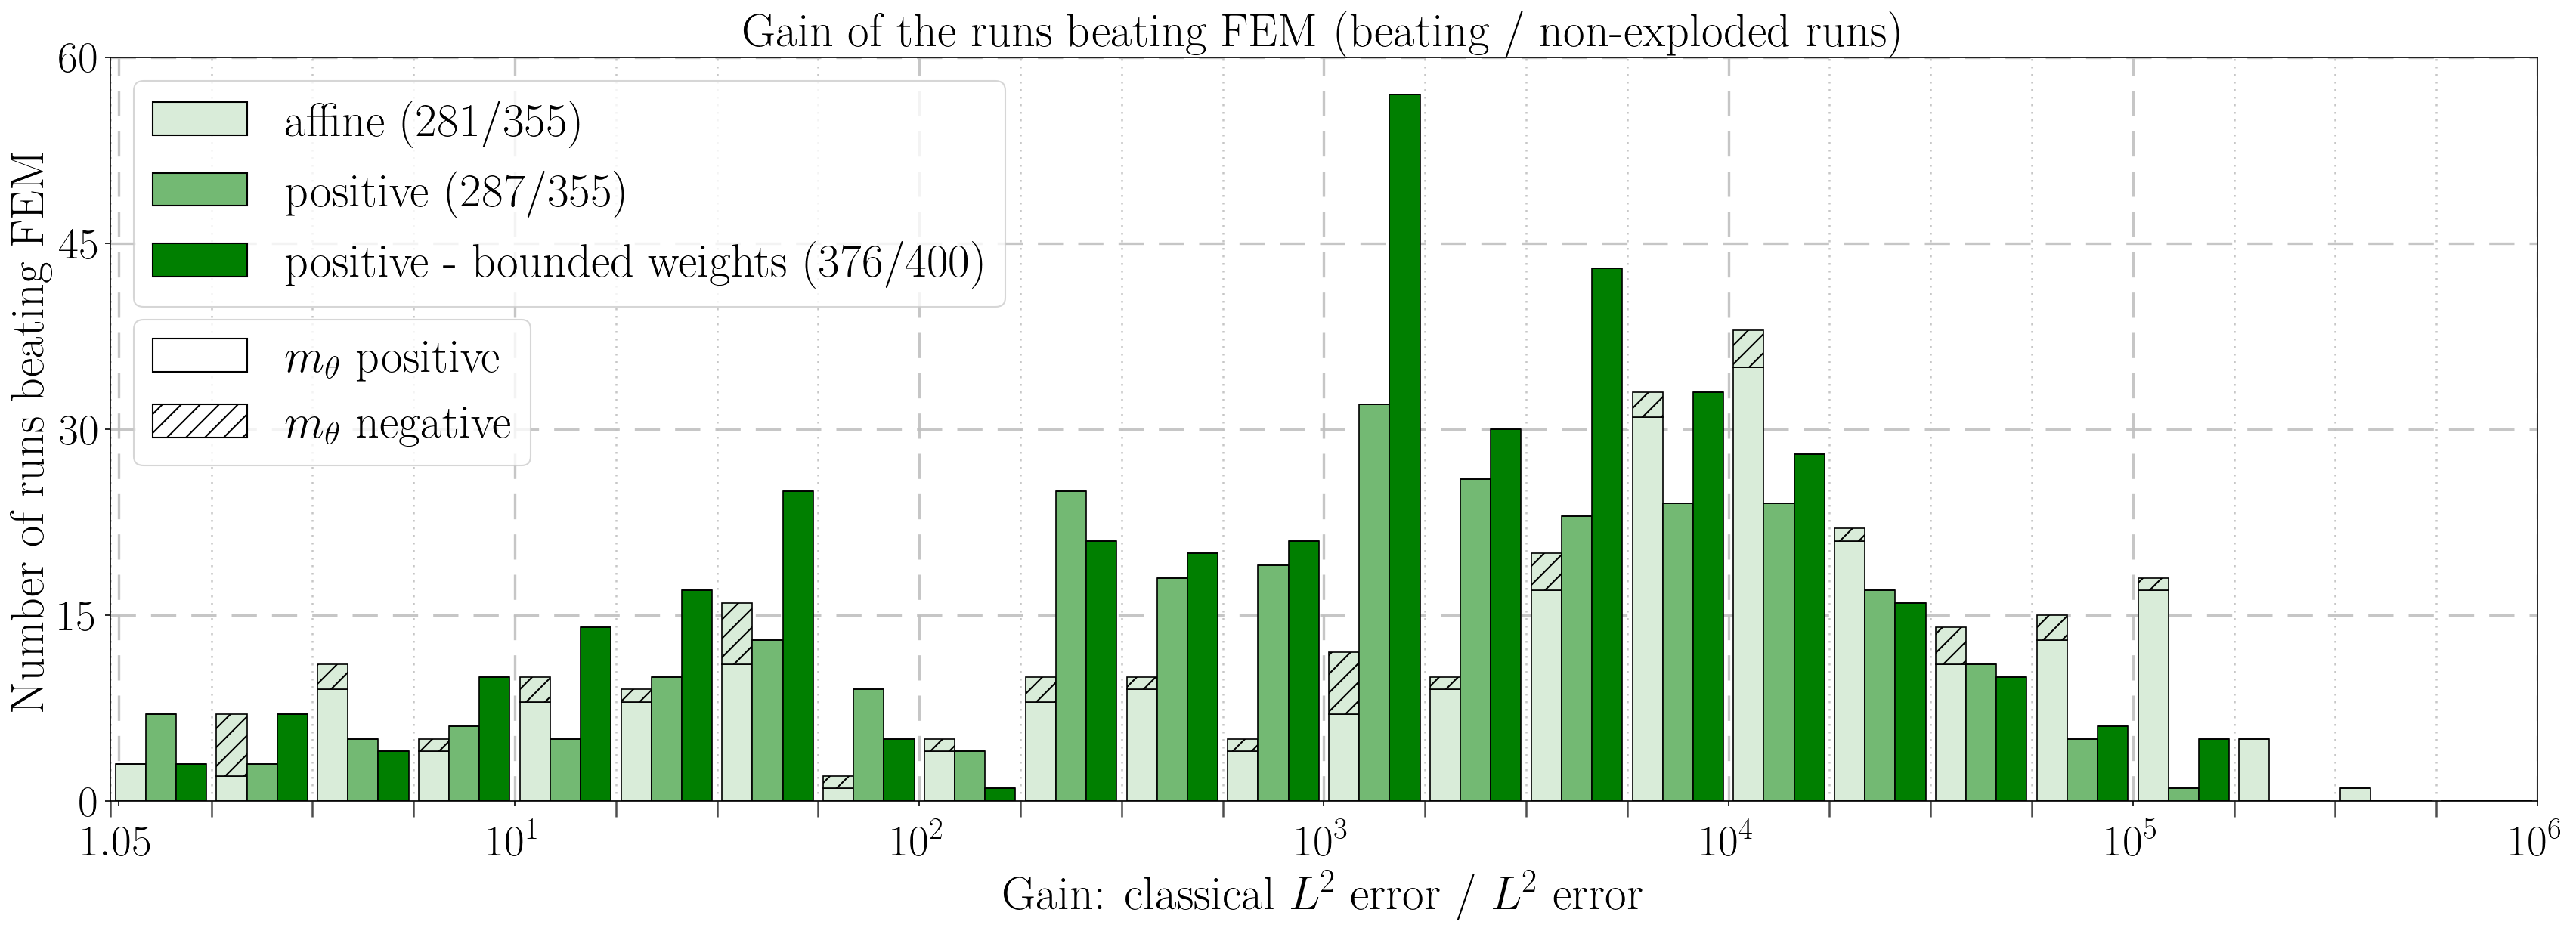
\includegraphics[width=\linewidth]{images/contrib2/multiplier/gain_distribution.png}}%
		\only<2->{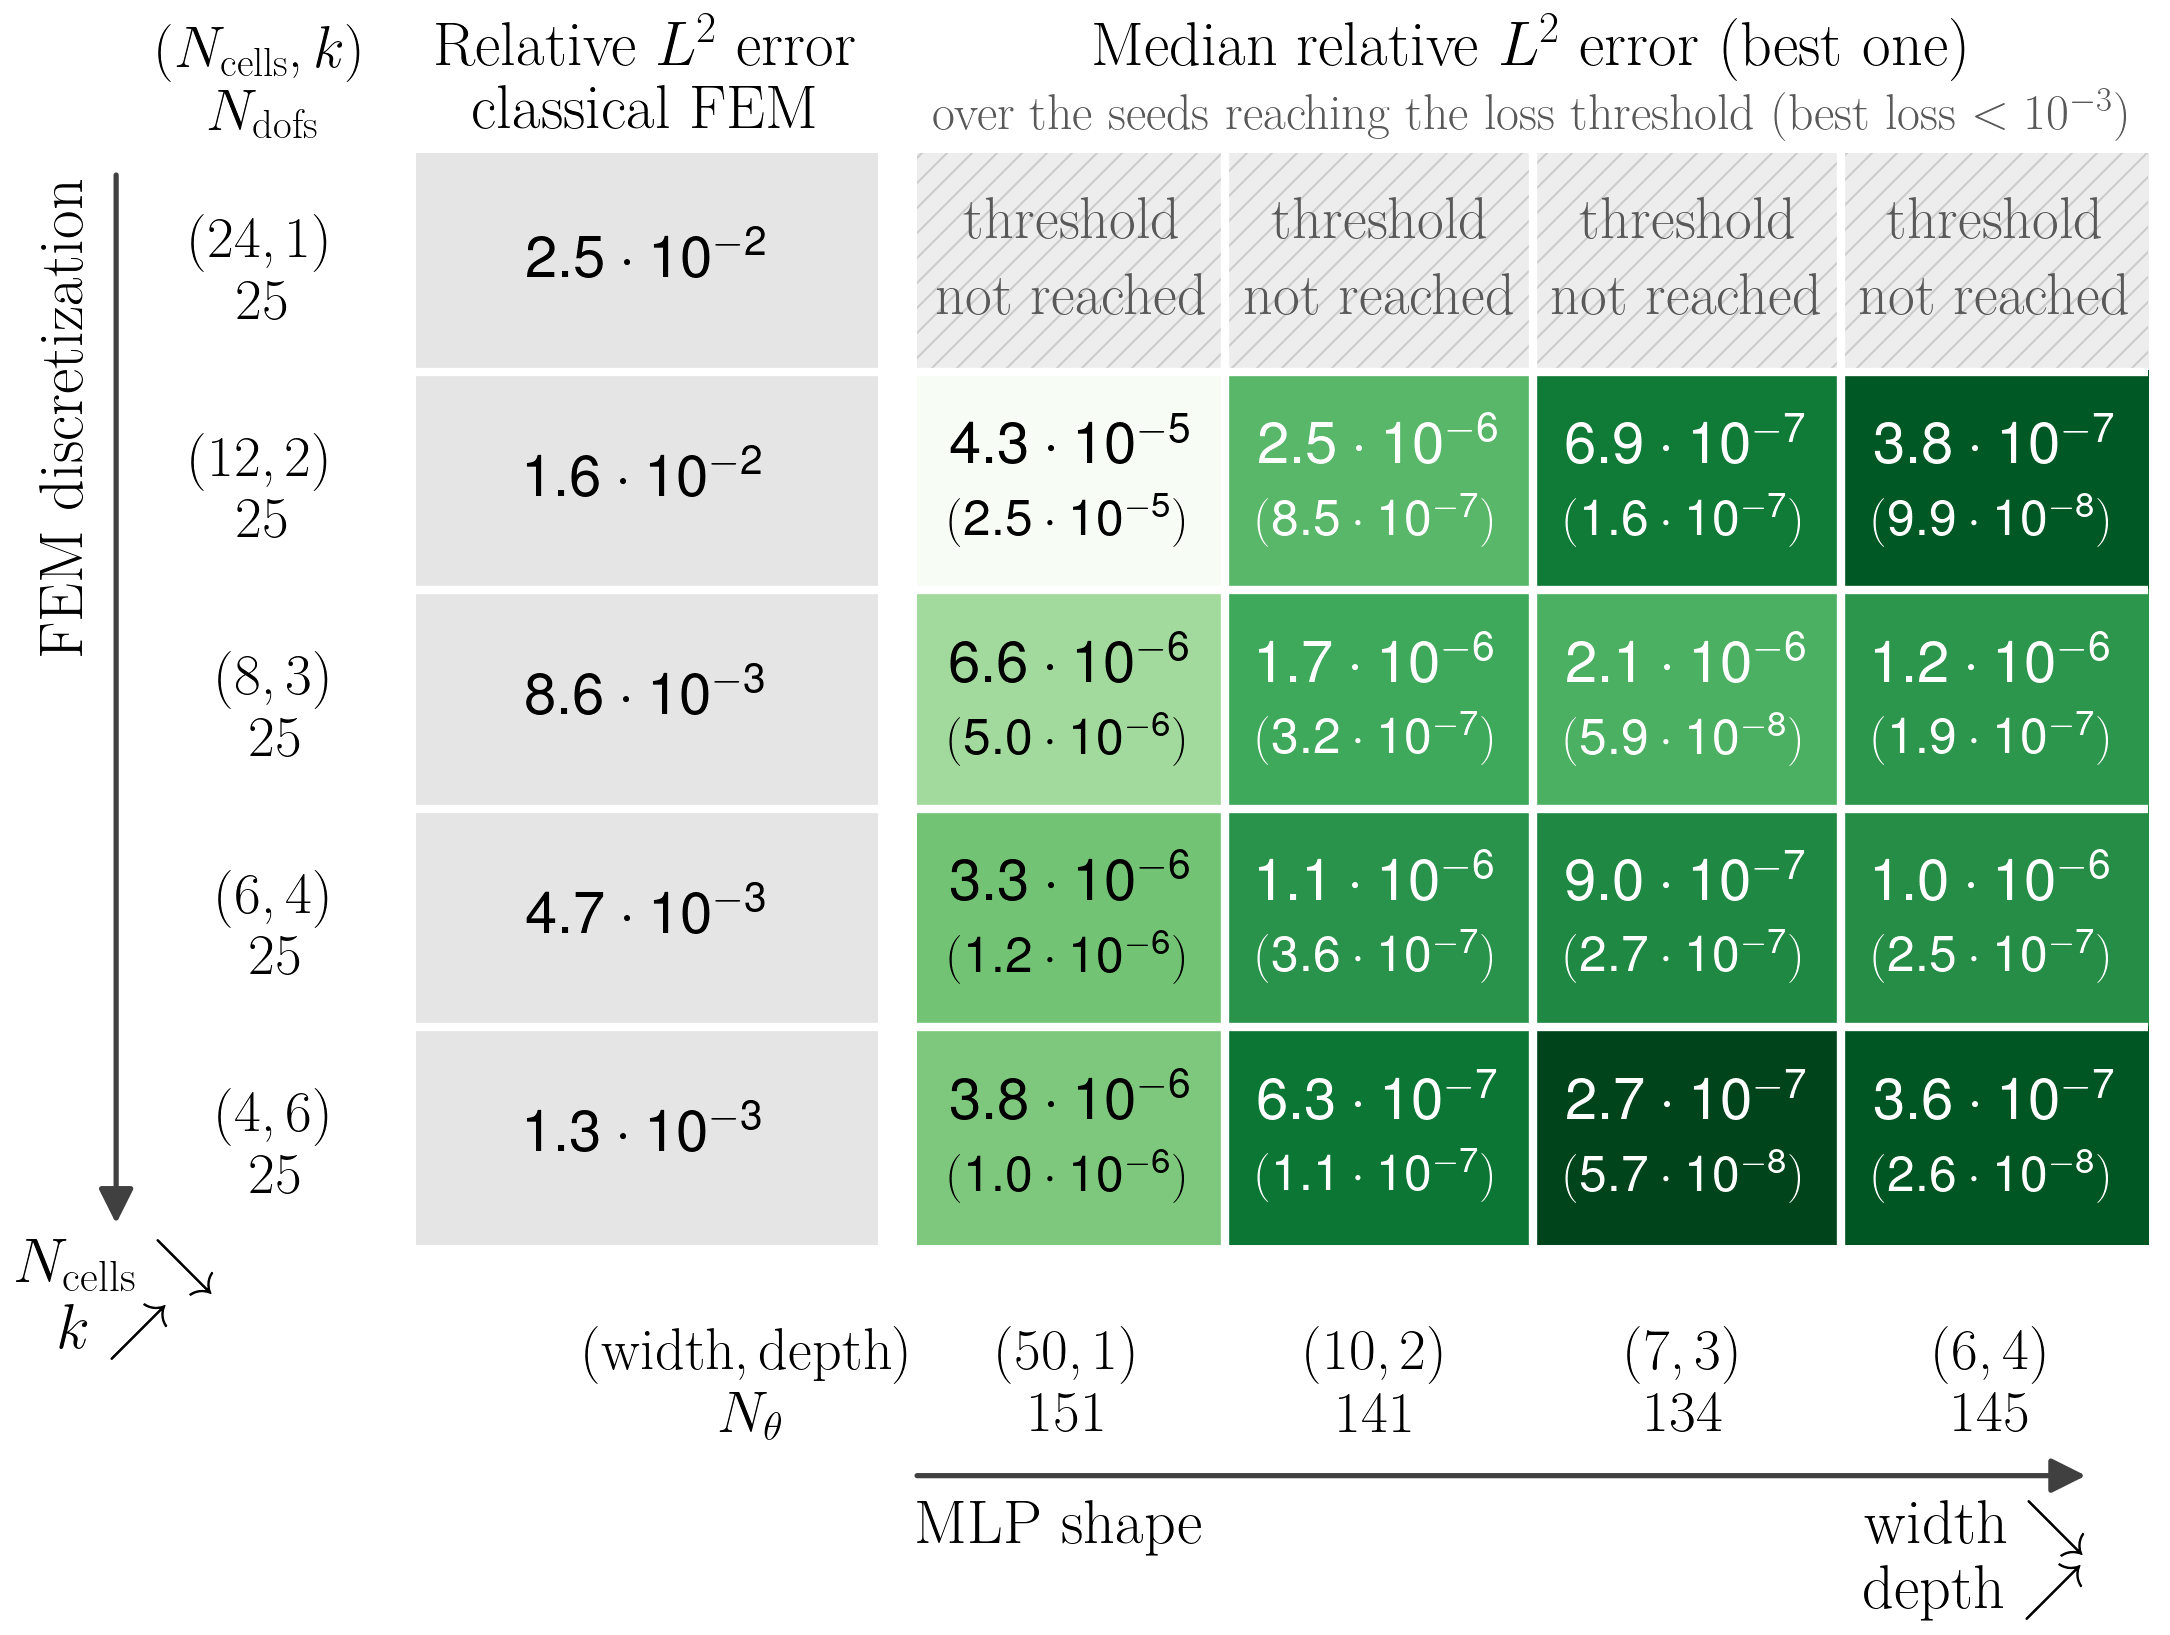
\includegraphics[height=5.6cm]{images/contrib2/multiplier/budget_summary_bounded_errors.png}}%
	}

	\vspace{7pt}
	\raggedright
	\textbf{Gain:} \coloredonly<1>{$376/400$} beat the FEM, none explodes; the affine multiplier keeps the highest gains.

	\vspace{4pt}
	\blk*{2}{%
		\textbf{Levers:} \coloredonly<2>{degree and depth matter}: $k=1$ only a modest gain over FEM, $(50,1)$ is the worst network.
	}
\end{frame}

\begin{frame}{3D test case}
	\rigiddisplayskips{7pt}
	\raggedright
	\textbf{Test case:} 3D advection-diffusion with a \coloredonly<1>{boundary layer}, $\Omega=(0,1)^3$, $\text{Pe}=20$:
	\vspace{-3pt}
	\[
		\left\{
		\begin{aligned}
			-\frac{1}{\text{Pe}}\,\Delta u+\bm{C}\cdot\nabla u & =f &  & \text{in } \Omega, \\
			u                                                  & =0 &  & \text{on } \Gamma,
		\end{aligned}
		\right.
		\qquad \bm{C}(\bm{x},\bm{\mu})=(\mu_1+\mu_2\,\bm{x}\cdot\bm{e}_\text{diag})\,\bm{e}_\text{diag},
	\]
	\vspace{-8pt}

	with $\bm{e}_\text{diag}=\frac{1}{\sqrt{3}}(1,1,1)^\top$ the diagonal direction and $\bm{\mu}=(0.8,0.8)$ fixed.

	\vspace{2pt}
	\blk{2}{%
		\textbf{Exact solution:} \coloredonly<2>{manufactured}, vanishing on the $6$ faces ($f$ deduced from it):
		\vspace{-3pt}
		\[
			u(\bm{x})=\prod_{i=1}^{3}x_i\Big(1-\exp\Big(-\frac{\text{Pe}\,(\mu_1+\mu_2)}{\sqrt{3}}\,(1-x_i)\Big)\Big)
		\]
	}

	\vspace{-3pt}
	\blk*{3}{%
		\textbf{Evaluation:} Relative $L^2$ error w.r.t.\ the manufactured solution $u$, \coloredonly<3>{never used in the training}.
	}
\end{frame}

\begin{frame}{3D: learned multiplier}
	\raggedright
	\textbf{Setting:} CG, $N_\text{cells}=4\times4\times4$ cells, $\mathbb{Q}_2$ ($N_\text{dofs}=729$), positive multiplier $m_\theta=\exp\big(6\tanh v_\theta\big)$.

	\textbf{Training:} MLP $v_\theta$ (tanh, $3\times10$, $N_\theta=271$), ENG optimizer, $70$ epochs, $6000$ collocation points, $3$ seeds.

	\vspace{-5pt}
	\parbox[t][4.6cm][c]{\linewidth}{\centering
		\only<2>{\animategraphics[autoplay,loop,palindrome,controls,poster=50,height=4.1cm]{12}{images/contrib2/pinn3d/anim_diagonal/f_}{00}{59}}%
		\only<3->{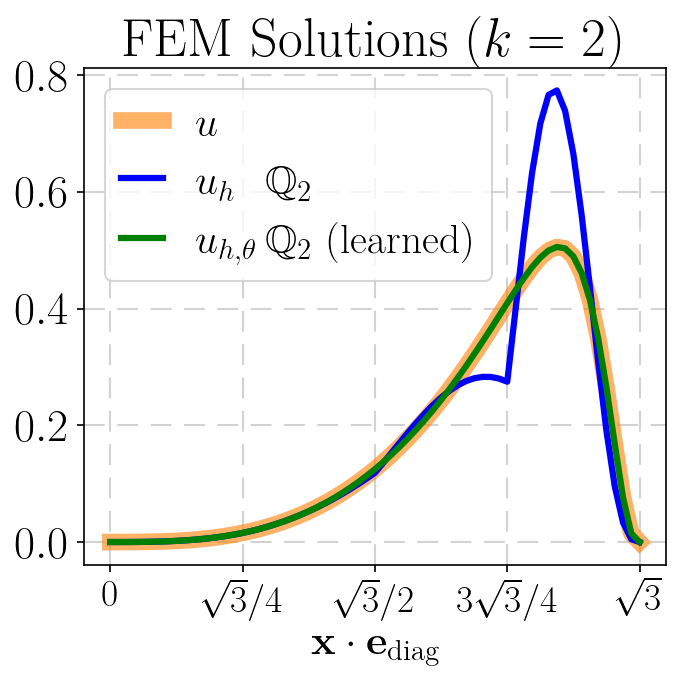
\includegraphics[height=4.3cm]{images/contrib2/pinn3d/diagonal_seed1_solution.png}\hspace{0.5cm}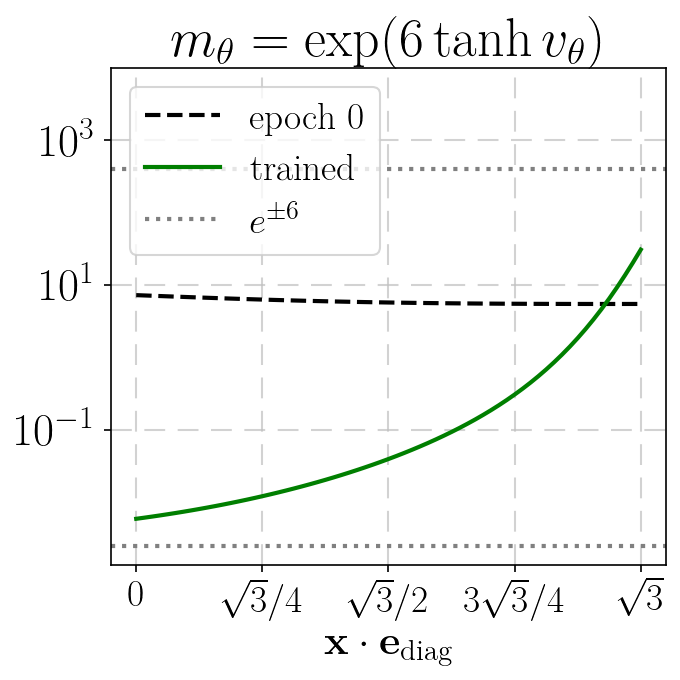
\includegraphics[height=4.3cm]{images/contrib2/pinn3d/multiplier_seed1.png}}%
	}

	\vspace{2pt}
	\only<2->{
		\textbf{Multiplier:} \coloredonly<2>{grows in the boundary layer}, from $6\cdot10^{-3}$ to $30$ (seed $1$).
	}

	\blk*{3}{%
		\textbf{Solution:} classical $u_h$ \coloredonly<3>{overshoots}, $u_{h,\theta}$ matches $u$.
	}
\end{frame}

\pgfplotstableread[col sep=comma]{images/contrib2/pinn3d/equal_time.csv}\PINNthreeDEqualTime % copie de equal_time.csv du manuscrit

\begin{frame}{3D: gain and cost}
	\parbox[t][3.0cm][c]{\linewidth}{\centering
		\small\setlength{\tabcolsep}{3pt}%
		\pgfplotstabletypeset[
			every head row/.style={
					before row={\toprule
							& \multicolumn{4}{c}{\textbf{time (s)}} \\
							\cmidrule(lr){2-5}
							& \multicolumn{2}{c}{\textbf{w/ comp.}} & \multicolumn{2}{c}{\textbf{w/o comp.}} & \multicolumn{3}{c}{\textbf{$N_\text{dofs}$}} & \multicolumn{3}{c}{\textbf{error}} \\
							\cmidrule(lr){2-3} \cmidrule(lr){4-5} \cmidrule(lr){6-8} \cmidrule(lr){9-11}
						},
					after row=\midrule,
				},
			every last row/.style={after row=\bottomrule},
			columns/seed/.style={column name={\textbf{seed}}, int detect},
			columns/t_learned/.style={column name={\textbf{learn.}}, fixed, precision=0},
			columns/t_classical/.style={column name={\textbf{class.}}, fixed, precision=0},
			columns/t_learned_run/.style={column name={\textbf{learn.}}, fixed, precision=1},
			columns/t_solve_run_classical/.style={column name={\textbf{class.}}, fixed, precision=1},
			columns/n_dofs_learned/.style={column name={\textbf{learn.}}, int detect},
			columns/n_dofs_classical/.style={column name={\textbf{class.}}, sci, precision=2},
			columns/ratio_dofs/.style={column name={\textbf{ratio}}, fixed, precision=0},
			columns/errL2_learned/.style={column name={\textbf{learn.}}, sci, precision=2},
			columns/errL2_classical/.style={column name={\textbf{class.}}, sci, precision=2},
			columns/ratio_error/.style={column name={\textbf{ratio}}, fixed, precision=1},
			columns={seed,t_learned,t_classical,t_learned_run,t_solve_run_classical,n_dofs_learned,n_dofs_classical,ratio_dofs,errL2_learned,errL2_classical,ratio_error},
		]\PINNthreeDEqualTime}%


	\vspace{8pt}
	\raggedright
	\textbf{Equal time:} error \coloredonly<1>{$\times6$ lower} for seeds $1$, $2$, equal for seed $3$.

	\vspace{2pt}
	\blk{2}{%
		\textbf{Dofs:} \coloredonly<2>{$534$ to $729$ times fewer} for the learned basis (without counting the $N_\theta=271$ weights).
	}

	\vspace{2pt}
	\blk*{3}{%
		\textbf{Cost:} learned time \coloredonly<3>{dominated by compilation}: $7$ to $10$ s without it, against $27$ to $50$ s for the FEM.
	}
\end{frame}
